Software guards our secrets, our money, our intellectual property,
our reputation \cite{covern}.  We entrust personal and
corporate information to software which works in an \emph{open} world, 
where  it interacts with % a vast number of
third party software of unknown provenance, possibly buggy and potentially malicious.

This means we need our software to be \emph{robust}.
We expect software to behave correctly even if  used 
by erroneous or malicious third parties.
 We expect that our bank will only make payments 
from our account if instructed by us, or by somebody we have authorized, 
that space on a web given to an advertiser will not be used
to obtain access to our bank details \cite{cwe}, or that a given
airline seat will only be sold once. 

The importance of robustness has led to the design of many programming
language mechanisms which help write robust programs:
constant fields, private methods, ownership\cite{ownalias}
as well as the object capability paradigm\cite{MillerPhD},
and its adoption in  web systems
\cite{CapJavaHayesAPLAS17,CapNetSocc17Eide,DOCaT14} and programming languages such as Newspeak
\cite{newspeak17}, Dart \cite{dart15}, Grace \cite{grace,graceClasses}, Wyvern \cite{wyverncapabilities}.

While such programming language mechanisms make it \textit{possible} to write robust
programs, they cannot \textit{ensure} that programs are robust.
Ensuring robustness is difficult because it means 
different things for different systems: perhaps
that critical operations should only be invoked with the requisite authority;
perhaps that sensitive personal information should not be leaked; 
or perhaps that resources belonging to one user should not be consumed by another.
%
To be able to ensure robustness, we need ways to specify what robustness means for the 
particular program, and ways to demonstrate that the particular program 
adheres to its specific robustness requirements.

There has been a plethora of work on the specification and verification of the
functional correctness of programs. Such specifications describe what are
essentially \emph{sufficient} conditions for some
effect to happen. For example, if you make a payment request to your bank, money will be transferred
and as a result your funds will be reduced: the payment request is a sufficient condition for the
reduction of funds. A bank client is also interested in \emph{necessary} conditions:
they want to be assured that no reduction in their funds will take place unless they themselves
requested it.

Necessary conditions are essentially about things that will  \emph{not} happen. For example,
if there should be no reduction to an account's funds without the
owner's explicit request, then that request being made by
the owner is the necessary condition for reducing funds - under no
other circumstances will the funds be reduced. 

We give a visual representation of the difference between sufficient and necessary conditions in 
Fig. \ref{fig:NecessaryAndSuff}. We
represent the space of all theoretically possible behaviours as points in the rectangle, 
each function is a coloured oval and its possible behaviours are the points in the area of that oval.  
The sufficient conditions are described on a per-function basis. 
The necessary conditions, on the other hand are about the behaviour of a module\footnote{\se{We use module and component in an analogous manner to class and object respectively.}} 
as a whole, 
and describe what is guaranteed not to happen;
they are depicted as black triangles. 

  \begin{figure}[htb]
 \begin{tabular}{ccccc}
\begin{minipage}{0.25\textwidth}
 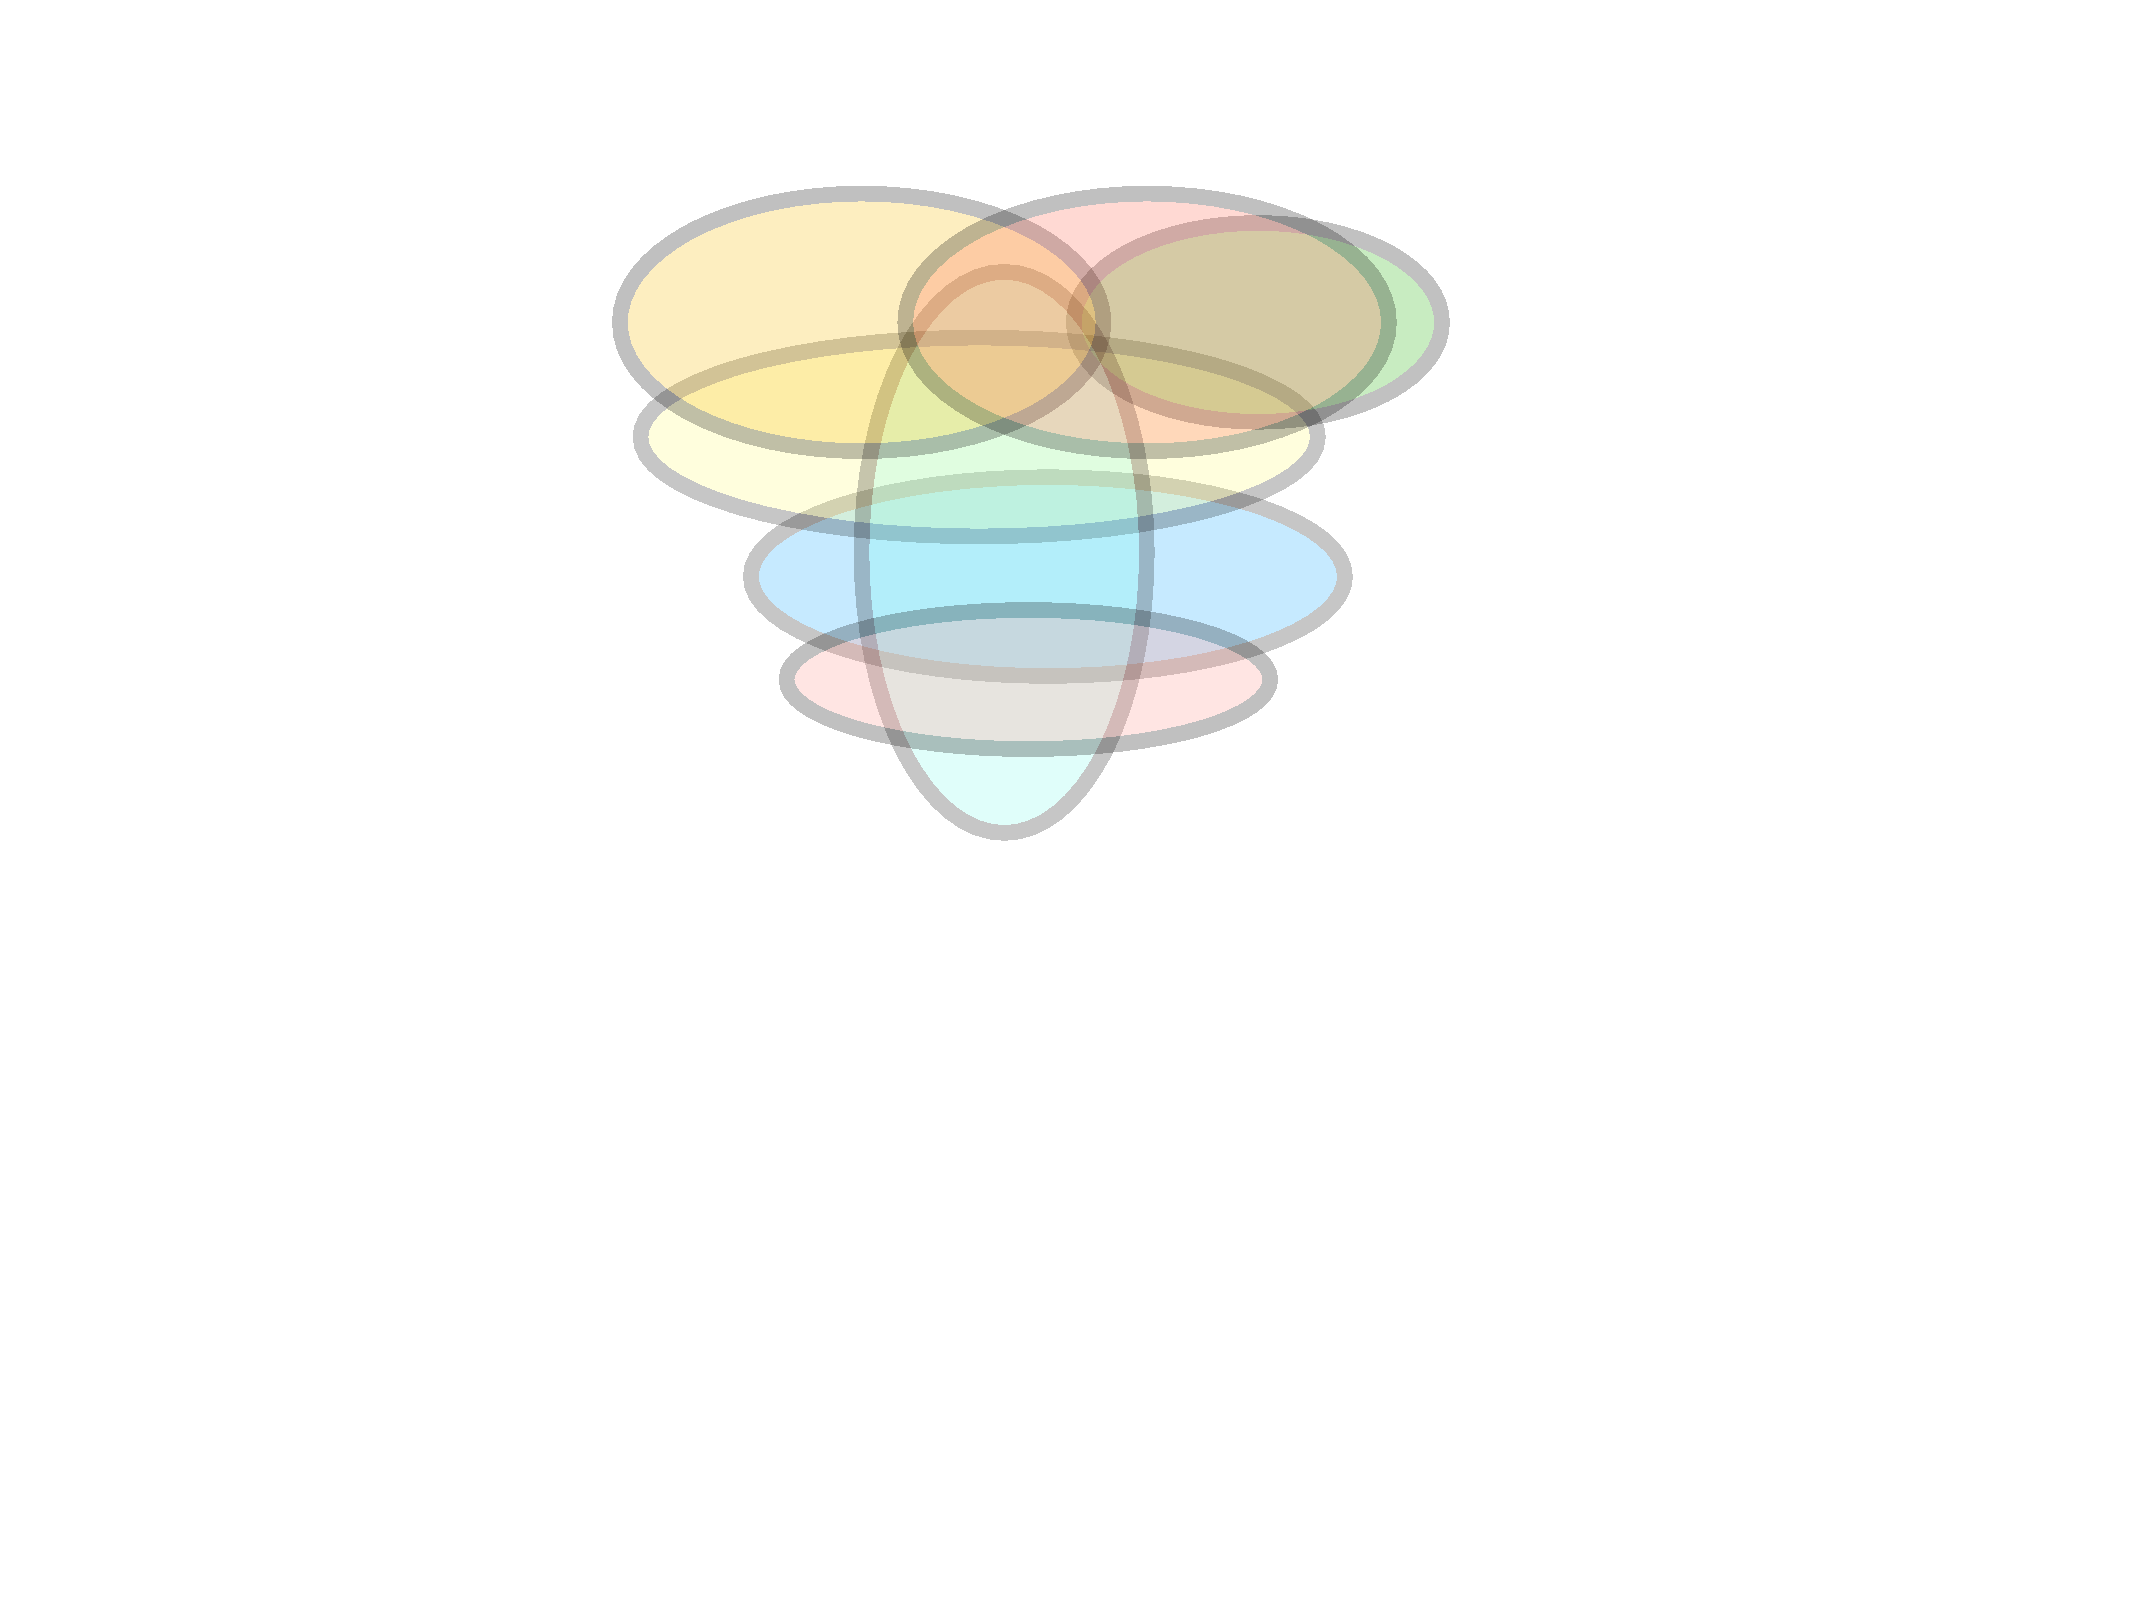
\includegraphics[width=\linewidth, trim=250  320 260 60,clip]{diagrams/Suff.pdf}
\end{minipage}
 & \ \ \ & 
\begin{minipage}{0.25\textwidth}
 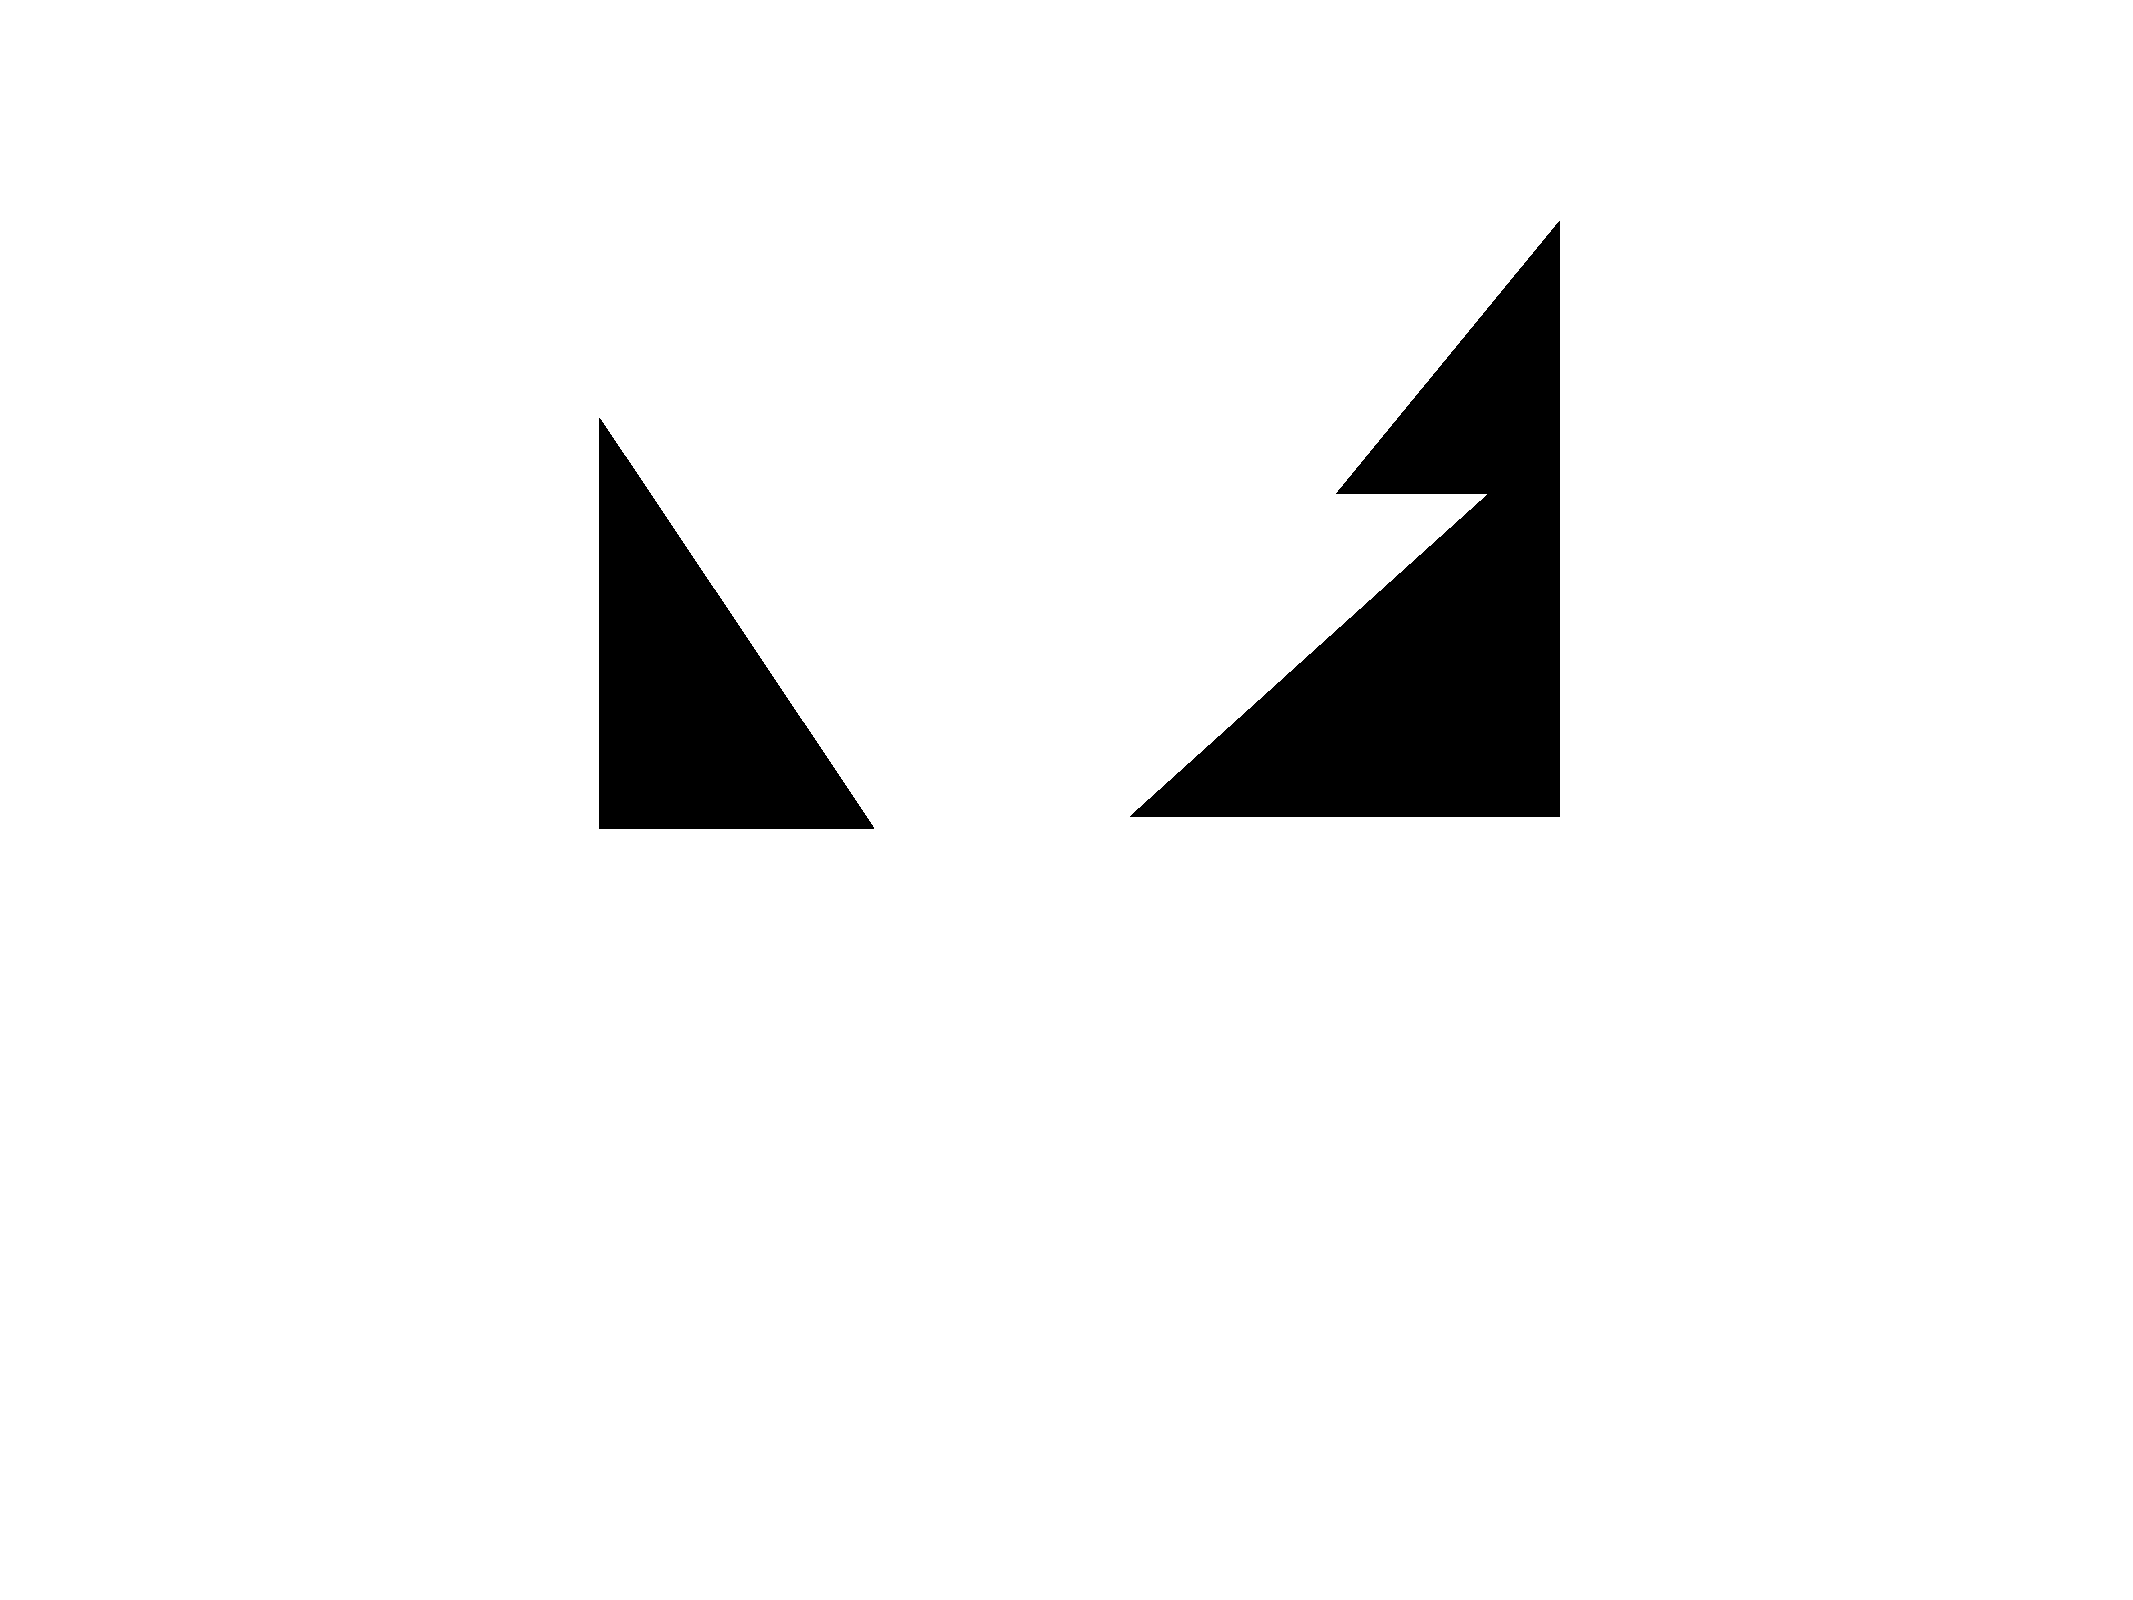
\includegraphics[width=\linewidth, trim=250  320 260 60,clip]{diagrams/Nec.pdf}
\end{minipage}
 & \ \ \ &
\begin{minipage}{0.25\textwidth}
 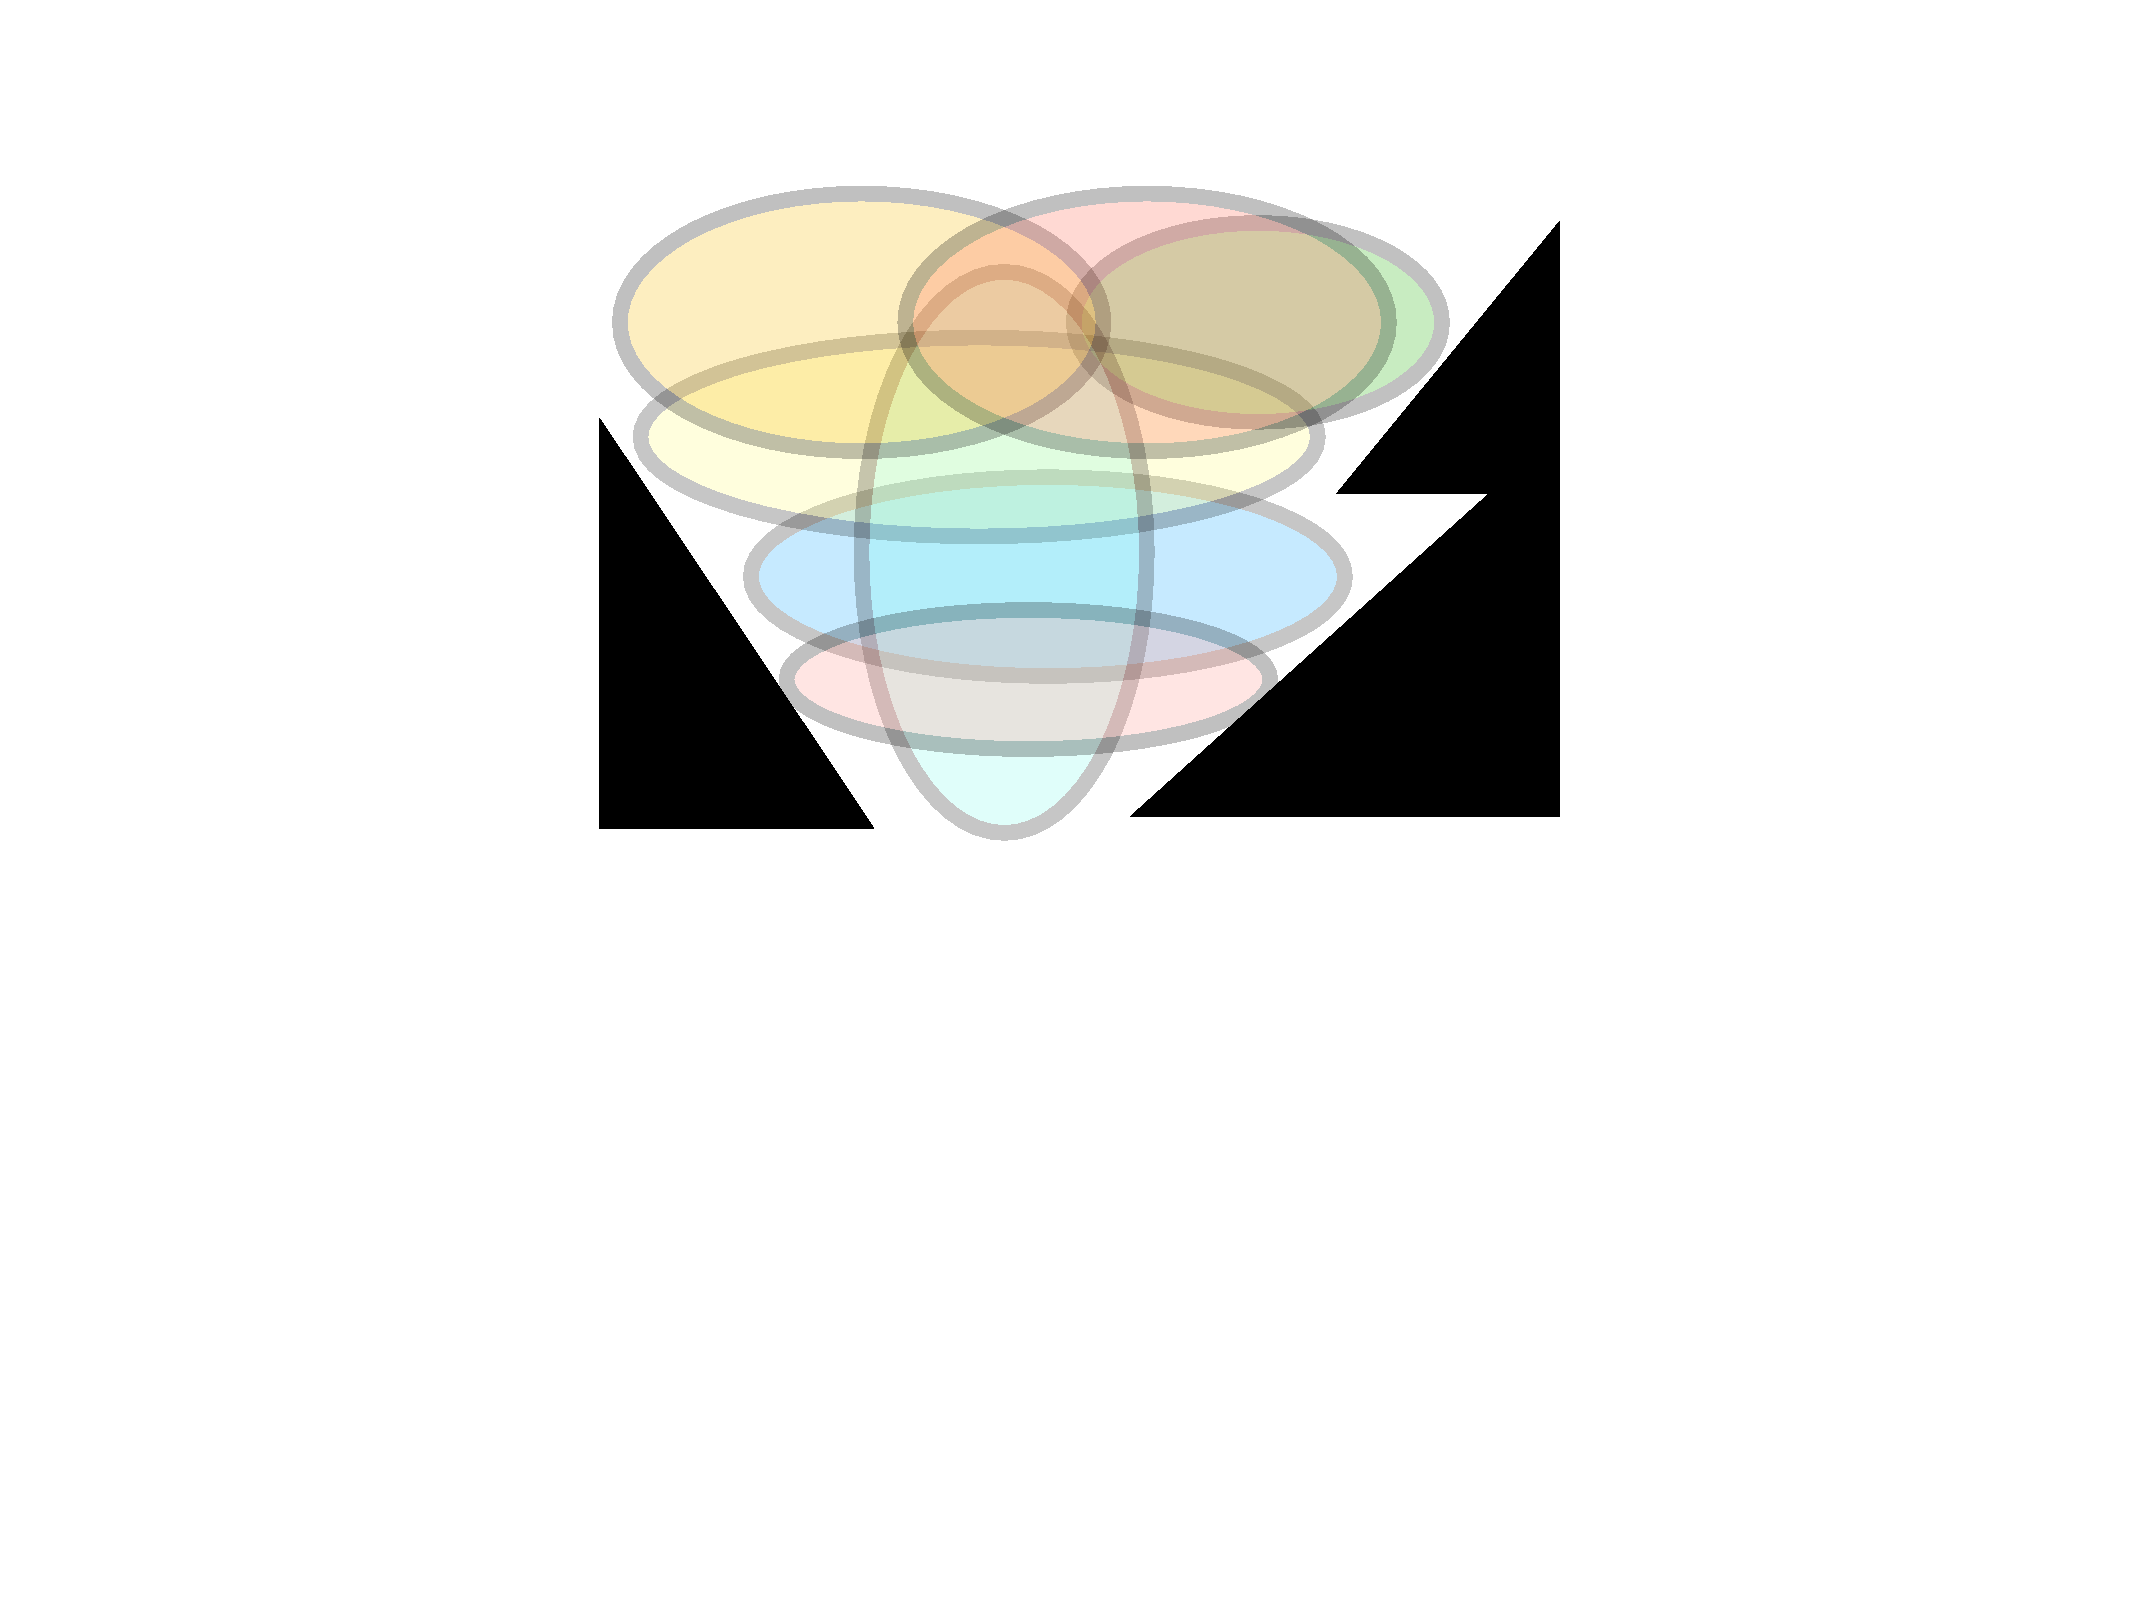
\includegraphics[width=\linewidth, trim=250  320 260 60,clip]{diagrams/NecAndSuff.pdf}
\end{minipage}
\\
sufficient  spec.& & necessary spec. & & holistic spec.
%\begin{minipage}{0.75\textwidth}
%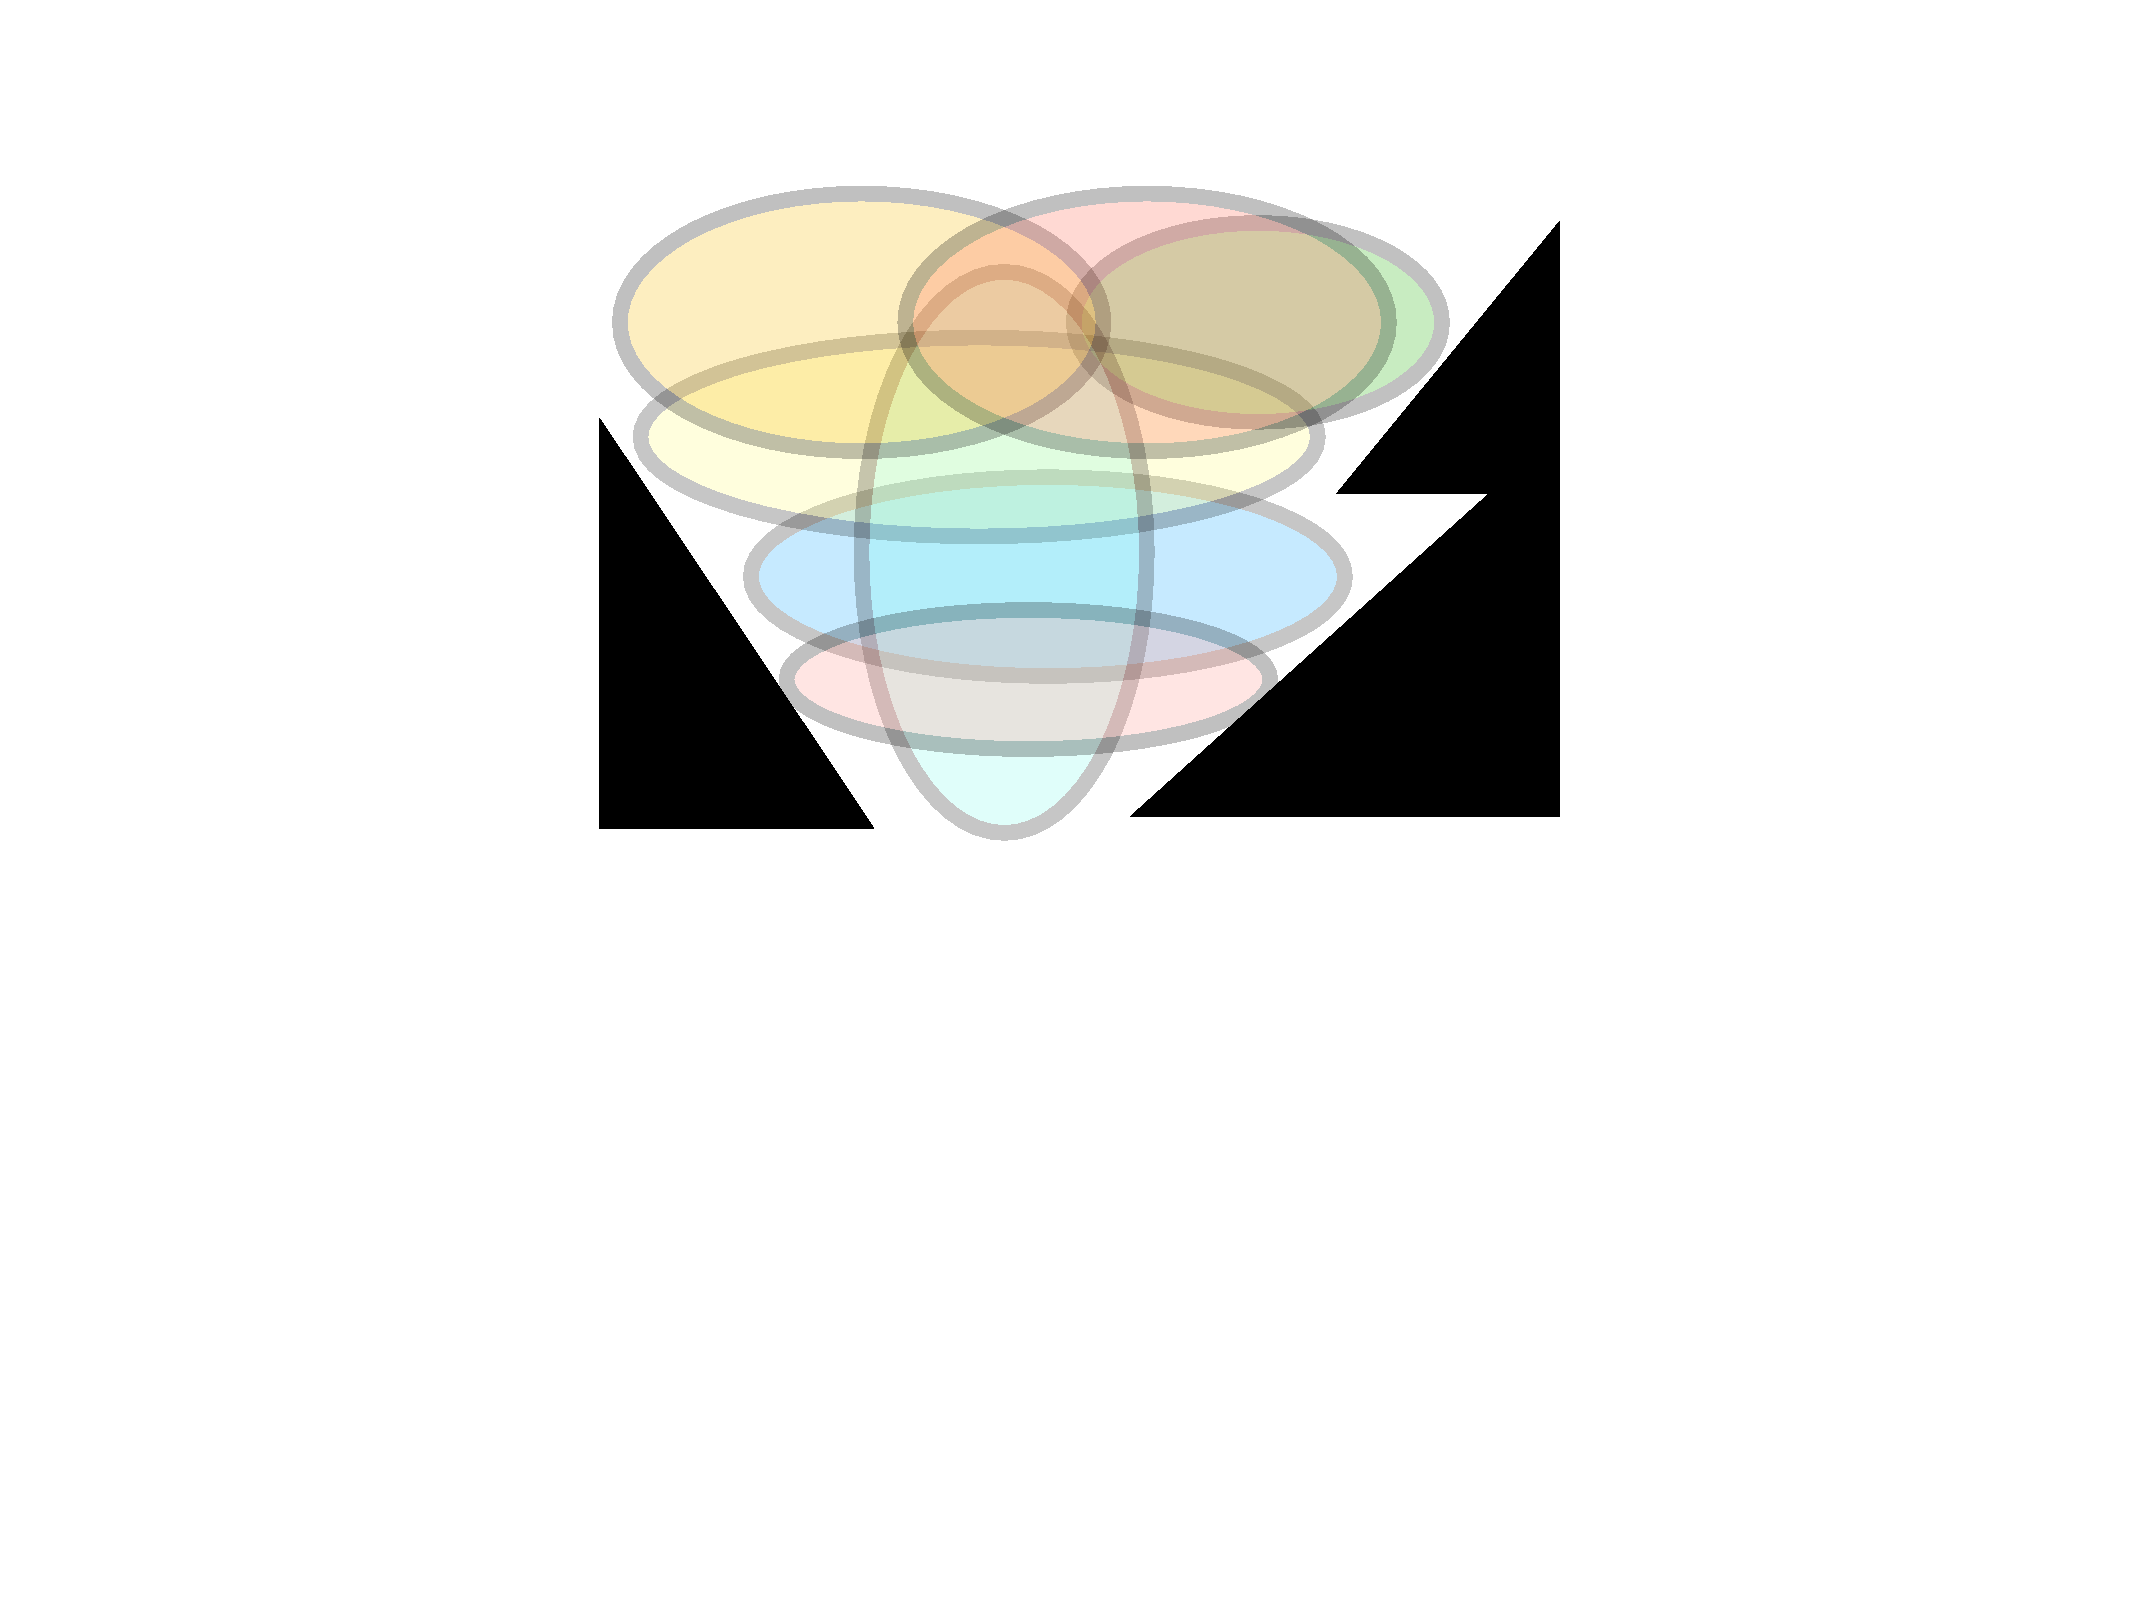
\includegraphics[width=\linewidth, trim=145  320 60 105,clip]{diagrams/NecAndSuff.pdf}
%\end{minipage}
%% y seems to eat up the bollom
%% x eats space from left, if you increase it the diagram decreases from left
%% w eats space from top, if you increase it the diagram decreases from top
%%\includegraphics[page=3, width=\linewidth, trim=150  270 40 150, clip]{diagrams/snmalloc.pdf}
%\sdcomment\sophia{I think we need to change the diagram so that it says small slab.}
%\end{minipage}
 \end{tabular}
  \vspace*{-2.5mm}
  \caption{Sufficient and Necessary Conditions, and Full Specifications}
 \label{fig:NecessaryAndSuff}
 \end{figure}
 
 We propose that  necessary conditions should be stated
 explicitly. Specifications should be \emph{holistic}, in the sense
 that they describe the  overall behaviour of a module: not only the
 behaviour of each individual functions, but also the 
 behaviour that emerges through combinations of functions.

Holistic specifications should therefore consist of   the sufficient as well as the necessary conditions, as  
depicted in right hand side  diagram in Fig. \ref{fig:NecessaryAndSuff}.
When a component has been specified holistically,  the behaviours
represented by the black triangles cannot occur, even when the
component interacts with other software of unknown provenance.
In Section \ref{sec:discussion} we argue why necessary conditions are more than the complement of
sufficient conditions.

Necessary conditions are guarantees upheld throughout program execution.
In this way, 
necessary conditions are closer to monitor or object
invariants \cite{Hoare74,Meyer97}. The difference between 
classical invariants and our holistic specifications is that classical invariants can only reflect  on
the current program state (\ie the contents of the
stack frame and the heap for an individual program component) while
holistic specifications reflect on all aspects of a program's
execution, potentially across all the components making up that program.


In this paper we propose \Chainmail, a specification language to
express holistic specifications.
%\james{has moved things around through here}
The design of \Chainmail was guided by the study of a sequence of
examples from the OCAP literature and the smart contracts world: the
membrane \cite{membranesJavascript}, the DOM \cite{dd,ddd}, the Mint/Purse \cite{MillerPhD}, the Escrow \cite{FTfJP14}, the DAO \cite{Dao, Daobug} and
ERC20 \cite{ERC20}.  As we worked through the
examples, we found a small set of language constructs that let us
write holistic specifications across a range of different contexts.
%
%
While many individual features of \Chainmail can be found in other work, 
their power and novelty for specifying open systems lies in their careful combination.
In particular, \Chainmail extends 
traditional program specification languages\cite{Leavens-etal07,Meyer92} with features which talk about:

\begin{description}
\item[Permission] Which object may have access to which other objects. 
Accessibility is central since access to an object usually also grants access to the functions it provides.

\item[Control] What object called functions on other objects. This is useful in identifying the causes of certain effects - eg 
funds can only be reduced if the owner called a payment function.

\item[Authority]  Which objects' state or properties may change. This is useful in describing effects, such as reduction of funds.

\item[Space] This is about which parts of the heap are considered when establishing some property, or when 
performing program execution and is
related to, but different from memory footprints and separation logics.

\item[Time] Assertions about the past or the future.
\end{description}


\james{moved around --- not sure we need this para}
\susan{I think we don't so there is a paragraph I have commented out.}
\forget{Formally, holistic assertions typically have the form of a guarantee
that if some property ever holds in the future, then some other property holds now.
For example, if within a certain heap some change is possible in the future, then this particular heap contains 
at least one object which has access to a specific other, privileged object.}
A module satisfies a holistic assertion if, for all other modules,
  the assertion is satisfied  in all runtime configurations reachable through execution of the two modules combined.
  This reflects the open-world view.


\noindent The contributions of this paper are:\kjx{can we claim each of these?}
\begin{itemize}
\item the design of the holistic specification language \Chainmail,
\item the semantics of \Chainmail,
\item a validation of \Chainmail through its application to a sequence of examples,
\item a further validation of \Chainmail through informal proofs of adherence of code to some of these specifications.
\end{itemize}  
  
  
The rest of the paper is organized as follows: Section~\ref{sect:motivate:Bank} 
motivates our work in terms of an example. Sections~\ref{sect:LangOO} contain a formal definition of \LangOO, and Section~\ref{sect:assertions} the semantics of assertions. Section ... related work .... Section xxxx concludes.
\kjx{TODO AT THE END}
